\begin{figure}[H]
	\centering
	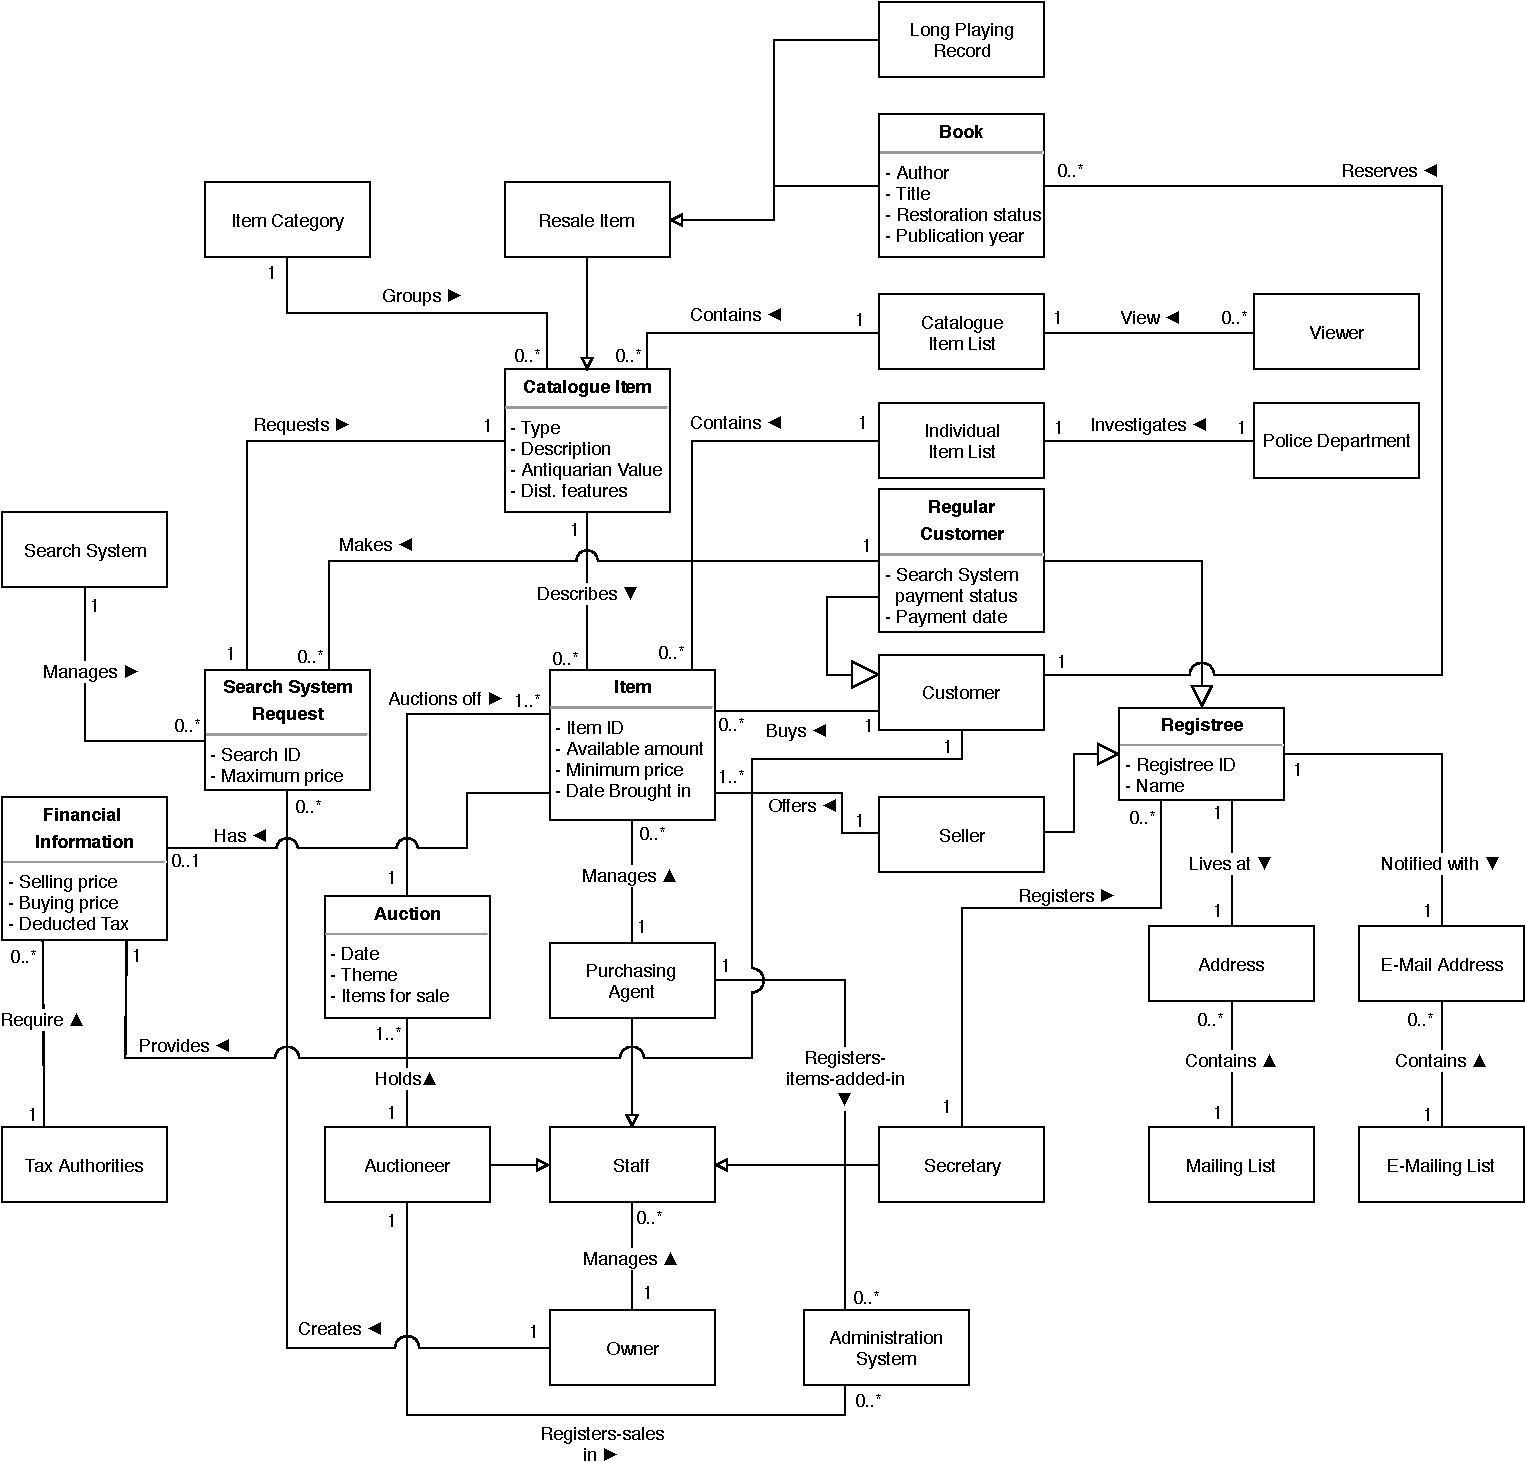
\includegraphics[scale=.9]{uml/domainmodelUPD3.pdf}
\end{figure}
% arrows for domain models to copy: ► ◄ ▲ ▼

% Things to add:
% Search Request, Book (maybe multiple kinds and a catalogue, well see)
The domain model is a universal, graphical representation of the relevant concepts and their attributes. It shows how all concepts relate to eachother.\\
For example, you can see that items are `used' by a number of sources, such as buyers, sellers, the auctioneer and the purchasing agent. Items are also described by a catalogue: a general form of the item to distinguish the individual item from the `item' as it is described. These catalogues are showed in an item list, which is just the collection of item catalogues available for purchase. The item list can in turn be viewed by the public.\\
Resale items are instances of catalogue items. These resale items specify an item that is often bought for resale. For example, books, which are in turn an instance of a resale item, are often bought up by small second-hand booksellers who offer the books for sale for more interested customers. To avoid selling expesive books for low prices, their value is estimated, which determines if they are sold to bookstores or kept in the storeroom.\\
We also see that all staff is an instance of the staff class. Any staff is then managed by the owner of The AuctionHouse\textsuperscript{TM}. This does not only make sense for our customer, but also for a future implementation, even though that is not (yet) our concern.\\
We see that a couple of parties can register something to the system. One is the secretary can add potential buyers and sellers to the system, granting them more permissions than the general public. Another is the purchasing agent, who can, after evaluation, add items to the system, making them available for viewing by the public.
There is no Auction concept in the domain model. The reason is that auctions are not going to be digitalized; they will still be physically held. Therefore, we do not concern ourselves with it when sketching the domain.\\
What remains is the ``Search System Request''. This is an entry for the search system, which is a service provided by the owner. The idea is that buyers can request to search for an item in The AuctionHouse\textsuperscript{TM}, or in a select group of other auctionhouses. The buyer can specify a maximum price he is willing to offer for the item. Whenever the owner find the item, he charges the buyer an amount depending on the price of the item. The service costs 20 euros a year.\\
The owner is the only one managing this service, so he is the only party who needs to interact with the requests.